% generated by scripts/pkl_to_latex.py
% source PKL : thermal_v1_L6_Ne6_U10_t1_mode-uniform_tpall_t2all_tperpall_nmin2_solver-gcg_sz0_restarts10_iter200_kmax4_tol1em09_cut10_adaptive1_step5_clusteravg1_T-205b87919d2f_knone_diag0.pkl
% scan type  : Tscan
% state      : gs
% requires   : \usepackage{pgfplots} \pgfplotsset{compat=1.18}
% colours match the matplotlib PDF (tab10 cycle)
\definecolor{gmeC0}{HTML}{1F77B4}
\definecolor{gmeC1}{HTML}{FF7F0E}
\definecolor{gmeC2}{HTML}{2CA02C}
\definecolor{gmeC3}{HTML}{D62728}
\definecolor{gmeC4}{HTML}{9467BD}
\definecolor{gmeC5}{HTML}{8C564B}
\definecolor{gmeC6}{HTML}{E377C2}
\definecolor{gmeC7}{HTML}{17BECF}

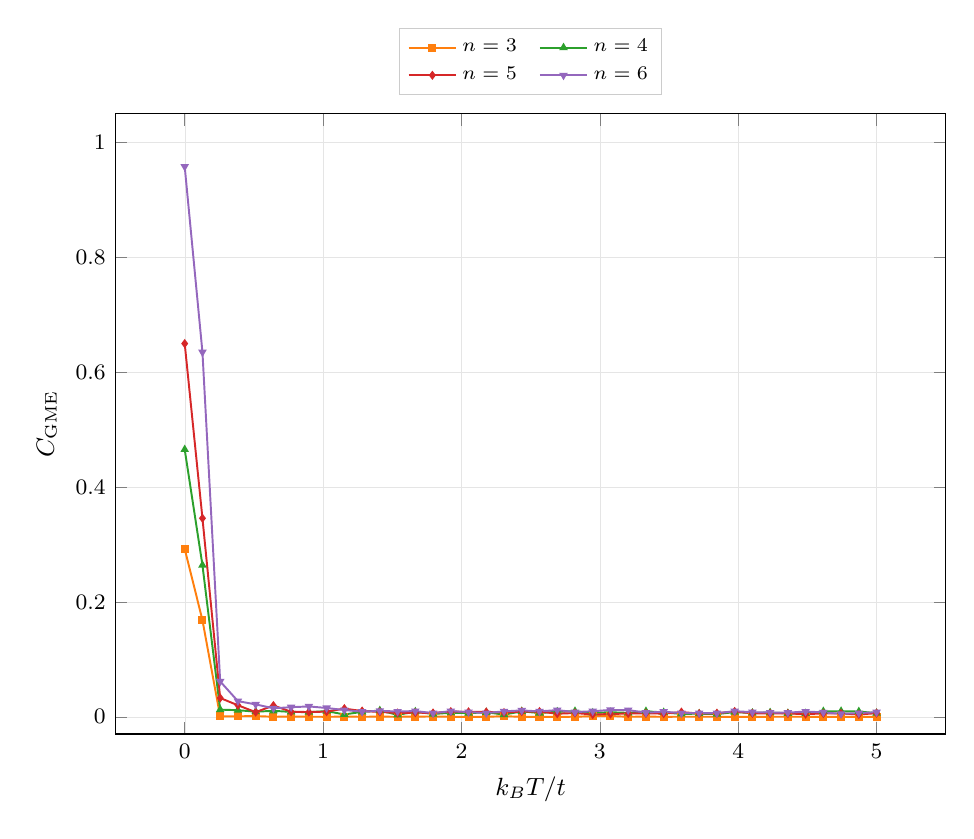
\begin{tikzpicture}
  \begin{axis}[
    width=\columnwidth,
    height=0.78\columnwidth,
    xlabel={$k_B T/t$},
    ylabel={$C_{\mathrm{GME}}$},
    grid=both,
    grid style={line width=.1pt, draw=gray!20},
    tick label style={font=\footnotesize\rmfamily, /pgf/number format/fixed},
    label style={font=\small\rmfamily},
    scaled ticks=false,
    legend style={font=\scriptsize\rmfamily, draw=gray!40, at={(0.5,1.03)}, anchor=south, /tikz/every even column/.append style={column sep=6pt}},
    legend cell align={left},
    legend columns=2,
    ymin=-0.03,
    ymax=1.05,
  ]
    \addplot[color=gmeC1, mark=square*, mark size=1.1pt, line width=0.7pt] coordinates {
        (0,0.292503) (0.128205,0.168318) (0.25641,0.00057) (0.384615,0.000871)
        (0.512821,0.0013) (0.641026,0.000111) (0.769231,0.000306) (0.897436,0.000172)
        (1.025641,0.000001) (1.153846,0.000366) (1.282051,0.000067) (1.410256,0.000288)
        (1.538462,0.000051) (1.666667,0.000398) (1.794872,0.00055) (1.923077,0.000007)
        (2.051282,0.000028) (2.179487,0.00004) (2.307692,0.001039) (2.435897,0.000022)
        (2.564103,0) (2.692308,0.000017) (2.820513,0.000061) (2.948718,0.00116)
        (3.076923,0.00143) (3.205128,0.000015) (3.333333,0.00037) (3.461538,0.000003)
        (3.589744,0.000095) (3.717949,0.000159) (3.846154,0.000019) (3.974359,0.000019)
        (4.102564,0.000001) (4.230769,0.000011) (4.358974,0.000197) (4.487179,0.000047)
        (4.615385,0.000006) (4.74359,0.000002) (4.871795,0.000015) (5,0.000005)
    };
    \addlegendentry{$n=3$}
    \addplot[color=gmeC2, mark=triangle*, mark size=1.1pt, line width=0.7pt] coordinates {
        (0,0.465514) (0.128205,0.264069) (0.25641,0.012486) (0.384615,0.011518)
        (0.512821,0.008904) (0.641026,0.010401) (0.769231,0.00854) (0.897436,0.008136)
        (1.025641,0.009884) (1.153846,0.004108) (1.282051,0.008657) (1.410256,0.010883)
        (1.538462,0.003481) (1.666667,0.008892) (1.794872,0.00485) (1.923077,0.00714)
        (2.051282,0.006391) (2.179487,0.007826) (2.307692,0.003894) (2.435897,0.009465)
        (2.564103,0.006593) (2.692308,0.008834) (2.820513,0.0097) (2.948718,0.006886)
        (3.076923,0.007926) (3.205128,0.006869) (3.333333,0.009547) (3.461538,0.007667)
        (3.589744,0.005055) (3.717949,0.00542) (3.846154,0.004784) (3.974359,0.008145)
        (4.102564,0.006661) (4.230769,0.007432) (4.358974,0.006079) (4.487179,0.00591)
        (4.615385,0.009489) (4.74359,0.009728) (4.871795,0.009177) (5,0.006432)
    };
    \addlegendentry{$n=4$}
    \addplot[color=gmeC3, mark=diamond*, mark size=1.1pt, line width=0.7pt] coordinates {
        (0,0.649931) (0.128205,0.345768) (0.25641,0.032775) (0.384615,0.02006)
        (0.512821,0.008132) (0.641026,0.019602) (0.769231,0.008869) (0.897436,0.008268)
        (1.025641,0.009029) (1.153846,0.014235) (1.282051,0.010029) (1.410256,0.008582)
        (1.538462,0.006577) (1.666667,0.007185) (1.794872,0.006738) (1.923077,0.008995)
        (2.051282,0.008711) (2.179487,0.008413) (2.307692,0.007306) (2.435897,0.009038)
        (2.564103,0.009124) (2.692308,0.005353) (2.820513,0.006616) (2.948718,0.004037)
        (3.076923,0.004822) (3.205128,0.005747) (3.333333,0.006005) (3.461538,0.005573)
        (3.589744,0.008252) (3.717949,0.00562) (3.846154,0.006319) (3.974359,0.009265)
        (4.102564,0.006122) (4.230769,0.005827) (4.358974,0.005719) (4.487179,0.0047)
        (4.615385,0.005801) (4.74359,0.005735) (4.871795,0.00406) (5,0.006357)
    };
    \addlegendentry{$n=5$}
    \addplot[color=gmeC4, mark=triangle*, mark size=1.1pt, mark options={rotate=180}, line width=0.7pt] coordinates {
        (0,0.958182) (0.128205,0.63501) (0.25641,0.061645) (0.384615,0.027294)
        (0.512821,0.021618) (0.641026,0.014868) (0.769231,0.016733) (0.897436,0.018073)
        (1.025641,0.015372) (1.153846,0.01177) (1.282051,0.009001) (1.410256,0.010385)
        (1.538462,0.009248) (1.666667,0.010011) (1.794872,0.006458) (1.923077,0.009838)
        (2.051282,0.008246) (2.179487,0.006503) (2.307692,0.009544) (2.435897,0.01112)
        (2.564103,0.009474) (2.692308,0.011693) (2.820513,0.008111) (2.948718,0.009752)
        (3.076923,0.011936) (3.205128,0.011744) (3.333333,0.007197) (3.461538,0.008929)
        (3.589744,0.006403) (3.717949,0.006507) (3.846154,0.00638) (3.974359,0.009781)
        (4.102564,0.008065) (4.230769,0.007471) (4.358974,0.007232) (4.487179,0.00923)
        (4.615385,0.00771) (4.74359,0.005088) (4.871795,0.006555) (5,0.007976)
    };
    \addlegendentry{$n=6$}
  \end{axis}
\end{tikzpicture}
